
% !TEX root = ../swputhesis.tex
\chapter{工作一:系统设计}
在本文第三章已充分阐述了所属方法的高效性,本研究在Win­dows场景下完成开发,采用编程语言 Python,并基于开发框架 PyQt5 和开发工具 Pycharm 进行开发。其中 PyQt5 框架是基于 Qt 框架的 Python 实现版本,其具有跨平台、库函数丰富和使用简单的特点。其可以运行在包括 Unix,Windows 和 Mac OS 平台上,能满足系
统的兼容性的需求。除此之外,涉及众多开源组件用于支撑整个项目的开发流程,包括PyTorch、Opencv­Python、NumPy、Scikit­learn 和 Matplotlib 等。最终实现对于图像分割效果查看,便于非专业用户对于所述方法的操作,实现该技术的生产应用。
\section{环境搭建}
本研究系统基于多个组件进行开发,组件的搭建主要分为以下步骤:
\begin{enumerate}
    \item 安装Anaconda与PyCharm。Anaconda是一个开源的Python发行版管理软件,内部收录了包含了许多科学计算库,PyCharm是一款捷克jetbrains公司开发的强大的Python集成开发环境。
    \item 安装与计算机匹配版本的CUDA 10.1和cuDNN。CUDA是NVIDIA推出的并行计算架构,cuDNN是CUDA深度神经网络库。要运行深度学习框架,CUDA和cuDNN的版本需与本机显卡相匹配(本研究显卡为NVIDA GeForce GTX 3060 Ti)。
    \item 配置更改环境变量。将CUDA的bin目录和lib目录添加到PATH环境变量中,将CUDA的include目录添加到CPLUS\_INCLUDE\_PATH环境变量中。该操作完成后,可以实现电脑全局调用CUDA加速包,便于后期模型推理计算使用。
    \item 安装PyTorch。PyTorch是一个基于CUDA的深度学习框架,可避免手动完成CUDA架构相关操作。本文使用PyTorch 1.8.1版本。此框架由facebook提出,因为可以实时调试的有点,许多计算机顶刊文章均基于PyTorch完成代码实现。
    \item 安装Cython、numpy、opencv-python、matplotlib、pillow、tensorboard、PyYAML、torchvision、scipy、 tqdm等其他库。这些库用于数据处理、可视化及其他操作。
    \item PyCharm上搭载Python 3.7解释器。选择File->Settings->Project Interpreter,点击“+”添加Python 3.8的Conda环境。
\end{enumerate}

完成以上步骤后,运行环境搭建完成。通过在Pycharm中运行示例程序,观察输出结果,确认环境配置正确。

\section{系统架构}
\subsection{系统总体设计}
针对系统的具体业务要求,本部分将对图像分割系统的整体结构进行梳理,实现系统总体架构设计,其体系结构如\cref*{fig:f4a}所示,主要分为三个模块:文件操作、图像分割和其他附加功能。其中文件操作模块负责处理文件上传和结果文件的输出,图像分割模块则调用本文第三章所属网络模型执行图像分割,展示分割结果。其他附加功能提供分类阈值自动设置,更改软件主题等功能,为用户提供更多的个性化选择。


\begin{figure}[htb]
    \centering
    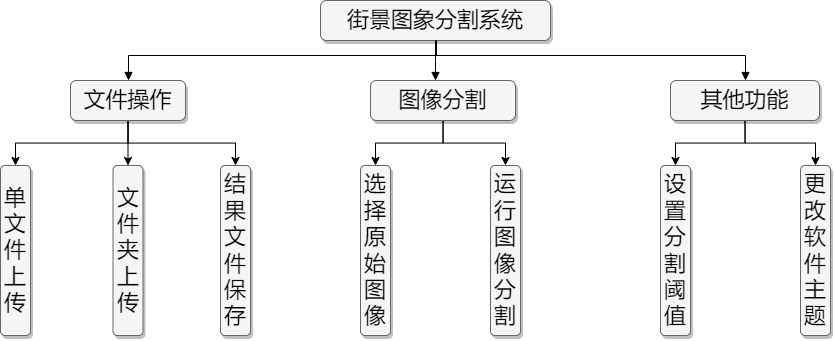
\includegraphics[width=12cm]{fig/chap4/系统架构图1.png}
    \caption{图像分割系统}
    \label{fig:f4a}
\end{figure}

\subsection{系统使用流程}
系统面向专业研究人员使用,为用户制定了具体的业务流程,简要的操作流程如\cref*{fig:f4b}所示。该系统不需要登录注册,仅作为轻量的图像处理工具,即插即用。用户直接进入系统主页面,根据需求上传图片文件或者图片文件夹。上传文件后,可对图像进行一系列基础图像操作,同时支持回退。也可以选择气泡检测功能,检测成功后系统会根据结果输出检测图像和计算的数据共同组成特征数据保存到本地。此上步骤均允许重复操作,每一步的操作结果均会显示在界面上。

\begin{figure}[htb]
    \centering
    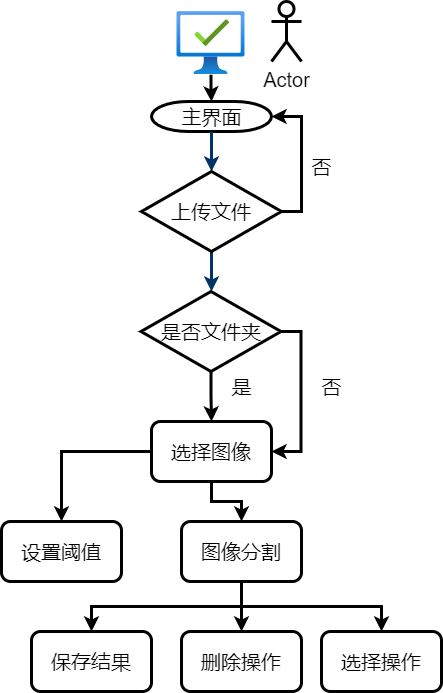
\includegraphics[width=8cm]{fig/chap4/系统流程图2.png}
    \caption{图像分割系统}
    \label{fig:f4b}
\end{figure}

\subsection*{文件操作}
文件操作模块主要涉及到文件上传和结果文件保存模块。文件上传模块提供单文件上传和多文件上传功能。用户选择单文件上传后,系统接收文件并计算图像的基本信息,
然后将这些信息回显到界面中。多文件上传是以文件夹的形式上传多张图像,系统为每张图像设置唯一编号,并在界面中显示编号列表以方便用户查看。
\subsection*{图像分割}
系统提供对所选择图像执行分割处理的操作,同时允许叠加多种图像处理操作,也支持回溯操作,即可以回退到上一步操作,防止用户误操作。用户可以根据最终的分割效果,对分割阈值进行调整,以获得更优的分割效果。
\subsection*{其他功能}
系统提供了软件主题明亮和暗黑的更新功能,软件主题的更换可以满足用户的个性化需求,实现定制化操作界面。 不同的主题可以带来全新的视觉体验,使软件界面显得更加新颖和时尚。主题更换增加了软件的趣味性,可以在一定程度上提高用户的体验度和依赖性。 相比功能更新,主题更换的成本较小,但可以产生较大的新鲜感,这在一定程度上延长了软件的生命周期。
\section{系统运行展示}
\cref*{fig:f4c}为所设计系统暗黑模式下的初始界面,居中部分为图像处理后结果的展示框,界面中下白色框展示图像路径,界面右下为操作按钮。\cref*{fig:f4d}展示了系统的执行过程效果图。
\begin{figure}[htb]
    \centering
    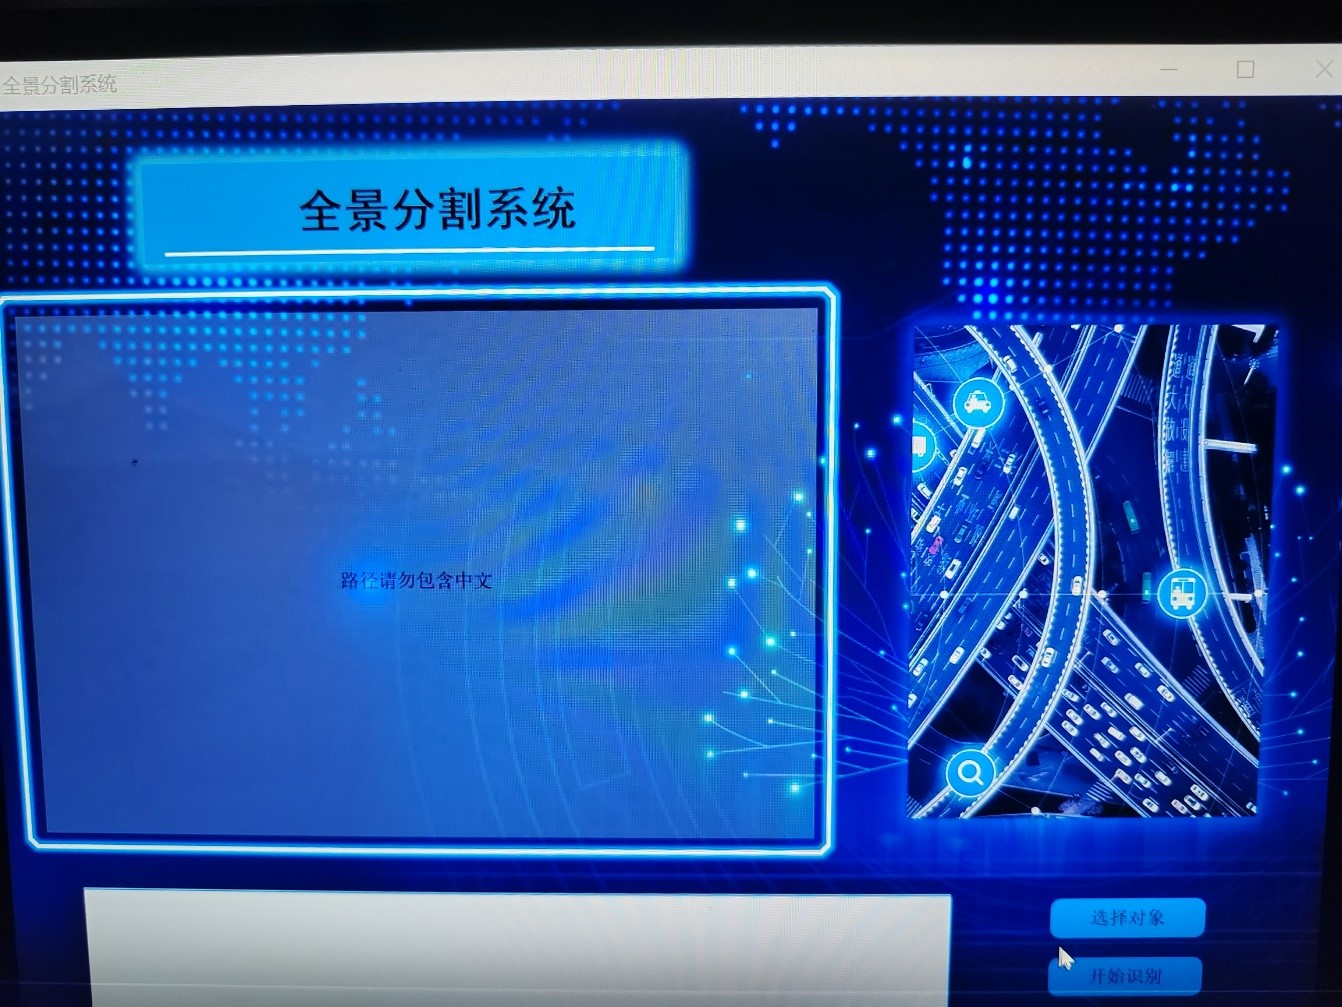
\includegraphics[width=8cm]{fig/chap4/可视化2.jpg}
    \caption{系统初始界面}
    \label{fig:f4c}
\end{figure}


\begin{figure}[htb]
    \centering
    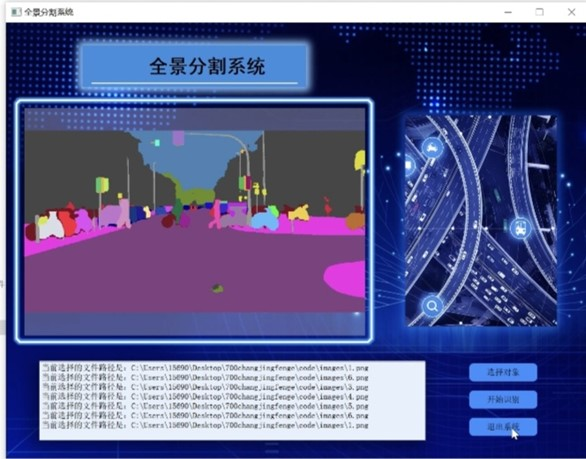
\includegraphics[width=8cm]{fig/chap4/可视化1.jpg}
    \caption{系统分割效果图}
    \label{fig:f4d}
\end{figure}
\subsection*{代码补充说明}
系统前端部分本研究采用PyQt完成软件开发,代码使用QtWidgets、QApplication等模块,编写代码中首先创建QApplication类的一个对象。这一步操作保证了UI应用程序存在入口点。然后使用本文创建QWidget类的一个对象。QWidget是Qt中所有UI对象的基类,本质上在应用程序中看到的所有东西都是一个小部件。包括对话框、文本、按钮、栏等等。官方允许用户设计复杂用户界面的功能,小部件嵌套完成堆叠效果。

系统模型部分,由于pytorch模型依赖于Pytorch框架,本研究为了减少平台依赖度,将PyTorch模型转换为了ONNX模型,ONNX是一个开放的神经网络交换格式,支持PyTorch、TensorFlow、Keras等主流深度学习框架之间的模型转换。转换为ONNX可以使PyTorch模型在更多平台下运行,不再限于PyTorch框架。ONNX模型可以部署到移动端和嵌入式设备。ONNX Runtime使ONNX模型可以高性能地运行在ARM、x86等服务器端和客户端CPU上,以及蓝牙等嵌入式设备上。这使得PyTorch模型得到更广泛的应用场景。ONNX模型具有较小的体积。相比PyTorch模型,ONNX模型提供了更加轻量级的格式,这使其更加适合在资源受限的环境下部署。
\begin{figure}[htb]
    \centering
    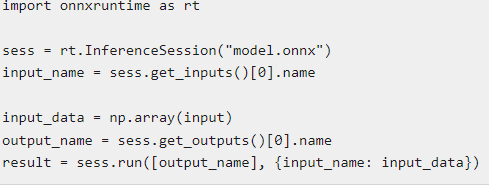
\includegraphics[width=8cm]{fig/chap4/代码图.png}
    \caption{加载ONNX模型实例代码}
    \label{fig:f4e}
\end{figure}

代码第一行,导入ONNX Runtime,用于加载和推理ONNX模型。 第二行,使用InferenceSession类加载ONNX模型。第三行,得到模型输入节点的名称。 第四行,构造模型输入数据。第五行,得到模型输出节点的名称。第六行,使用run方法进行模型推理,输入数据传入输入节点,输出数据从输出节点获得。第七到第十行,输出模型推理结果。



\section{本章小结}
为了更方便研究人员快速、便捷的利用所属的深度学习模型对街景图像的分割处理,帮助后续执行自动驾驶追踪。本章利用 PyQt5 框架,设计开发了一个图像分割系统。系统实现了诸如文件操作、图像分割和其他附加功能,可供专业研究人员快速对街景图像进行处理,同时获取相关图像特征,以便后续利用这些特征与自动驾驶获得的其他特征信息进行建模。
